\section{Network Structures}

Just like stock markets and airline routes, the cyber-insurance market can be described using graphs. The structure that will evolve is dependent on all the nodes and how they connect with each other. The insurer can determine the cost of establishing a link, and thus  determine which nodes will connect to eachother. This is what we will try to achieve in our models. However, first we need to shed light on what kind of graph structures that would be desirable to force upon the cyber-insurance market.

To find the proper structure, many different scenarios should be covered. In a network an agent's actions are influenced by its neighborhood structure, i.e. the network connections will affect each individual agent's payoff, meaning that agents are dependent on eachother, and the probability of cascading failures are highly relevant. -If one or more fails, e.g. bankruptcy, failure to deliver at the expected time, system shut down, higher cost etc, then the whole network will be affected. In this case there are several types of networks to consider, every social and economic interaction where an agent's well-being is dependent on externalities as well as on his own actions, is a network worth considering.

We found several interesting papers from evolutionary studies and disease epidemics, which described  characteristics in different graph structures. The ones we found appropriate, were those which described the benefits of star- and clique-shaped graphs. These graphs showed characteristics that could be used to make it feasible for both the insurer to offer - and the customer to acquire insurance. 

 The paper \cite{lieberman2005evolutionary} is about evolutionary dynamics and how some structures
can amplify or sustain evolution and drift\footnote{Drift is the opposite of selective evolution, it is when the network/structure evolve and change at random}. One aspect of cyber-insurance is risk, and knowledge of how, for example, viruses spread in a network and how to use graph structures to prevent both hackers from entering and virus from spreading, is important. Evolutionary dynamics, and the research of how mutant genes spread throughout a population, as described in the paper, is analogous to this issue.
If we can determine some structures where certain nodes are advantageous/disadvantageous, then these structures will have imporant  properties, such as sustaining viruses from spreading, or amplify the incentive for obtaining cyber-insurance. 

The paper \cite{lieberman2005evolutionary}, shows that mutants inserted into a circulation graph, will have a fixation probability equal to
\begin{equation}  
p_{1}=\frac{(1-\frac{1}{r})}{(1-\frac{1}{r^{N}})}
 \label{eq:fixation} 
\end{equation}
Where $r$ represents the relative fitness of the mutant i.e the agents security level, if it is advantageous it will have a certain chance of fixation, and disadvantageous mutants will have a chance of extinction. A circulation graph is a graph that satisfies these two properties: 
\begin{enumerate}
\item The sum of all edges leaving a vertex is equal for all vertices
\item The sum of all edges entering a vertex is equal for all vertices
\end{enumerate}
A clique is a good example of a circulation graph, and the probability of fixation is as in Eq. (\ref{eq:fixation}).
The fixation probability determines how probable it is that the whole network will eventually be
"infected" by the mutant. Which means that it determines the rate of evolution, which relies on both the size of the
network and the evolution speed. 
If the relative fitness of the nodes is high, then the probability of fixation will be low.
A probability equal to one means that every node in the network will eventually be affected by the mutant.

An essential part of cyber-insurance is as mentioned earlier, for the insurer to be able to calculate the overall risk of the instance to be insured. Since the probability of fixation can be calculated in circulation graphs, if the insurer knows that the instance is part of a circulation graph, it is possible for the insurer to calculate the probability of fixation in that network. 
If we can find graphs with a fixation probability that exceeds Eq.(\ref{eq:fixation}) it is even better, because then the insurer is not only able to calculate the overall probability of fixation, but also to show that the probability of fixation is higher than the one for circulation graphs.
\begin{figure}[b]
\centering
\begin{tabular}{@{}c@{}}
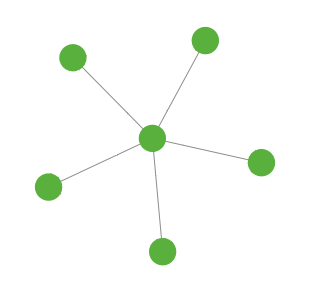
\includegraphics[width=0.5\textwidth]{../Figures/aStar.png}
\end{tabular}
\caption[A start structure]{
\label{fig:star} A star topology. 
}
\end{figure}
\cite{lieberman2005evolutionary} shows that such graphs exist, and one example is the star topology, (see Figure \ref{fig:star}).
In this topology the fixation probability is as shown in Eq.(\ref{eq:fixation2}), or more generally Eq.(\ref{eq:fixationk})\footnote{The parameter $k$ is an amplifier parameter. The star structure is a $k=2$ amplifier, and the super-star, meta-funnel and funnel  can all be extended to arbitrarily large $k$, thereby guaranteeing fixation of any advantageous mutant \cite{lieberman2005evolutionary}.}. \begin{equation}p_{2}=\frac{(1-\frac{1}{r^{2}})}{(1-\frac{1}{r^{2N}})} \label{eq:fixation2} \end{equation}.

\begin{equation}
p_{k}=\frac{(1-\frac{1}{r^{k}})}{(1-\frac{1}{r^{kN}})} \label{eq:fixationk}
\end{equation}
 When comparing Eq.(\ref{eq:fixation}) and Eq.(\ref{eq:fixation2}), we see that the selective difference is
 amplified from $r$ to $r^{2}$, i.e. a star acts as an evolutionary amplifier, favoring advantageous
  mutants and inhibiting disadvantageous mutants.

There are other graphs where the fixation probability is equal to \ref{eq:fixationk}, examples are super-stars, such as funnels and
metafunnels. These are just more complex star networks. This paper shows that as N gets large, the super-stars will have a fixation probability, for an advantageous mutant, that converges to 1, and for a disadvantageous mutant converges to 0. 
As exemplified earlier in this chapter, we know that there are many
topologies in our society that are so called scale-free graphs. These graphs have most of their connectivity clustered in a few vertices, which are very similar to a network interconnected by multiple stars, these networks can also be considered as potent selection amplifiers. 


The paper \cite{contagion} present interesting results regarding network formation games. 
The authors set up a game where the nodes benefit from direct links, but these links also expose them to risk. 
Each node gains a payoff of $a$ per link it establishes, but it can establish a maximum of $\delta$ links.
A failure occurs at a node with probability $q$, and propagates on a link with probability $p$. If a node fails, it will receive a negative payoff of $b$, no matter how many links it has established. The characteristics of this game is transferable to how we expect nodes in a cyber-insurance network to interact with eachother. Therefore, the results of the overall payoff change according to different collection of participants. 

The results from the model presented by Blumen et.al. shows a situation where clustered graphs achieve a higher payoff when connected to trusted nodes, compared to when connecting with random nodes. Unlike in anonymous graphs, where nodes connect to each other at random, nodes in these graphs share some information with their neighbors, which is used when deciding whether to form a link or not. 
To further explain these results, they show that there exists a critical point, called \textit{phase transition}, which occurs when nodes have a node degree of $\frac{1}{p}$. 
At this point a node gets a payoff of $\frac{a}{p}$, and to further increase the payoff the node needs to go into a region with significantly higher failure probability. 
Because once each node establishes more than $\frac{1}{p}$ links, the contagious edges will with high probability form a large cluster, which results in a rise in probability of node failure, and reduces the overall welfare.
From this the paper states that when the minimum welfare exceeds 
$(1+f(\delta)*\frac{a}{p})$
we have reached \textit{super-critical payoff}. Otherwise it is called \textit{sub-critical payoff}. 
Further Easley et.al, show that the only possible way of ending up with super critical payoff, is by forming clustered networks consisting of cliques with slightly more than $\frac{1}{p}$ nodes. 
However, if the nodes form an anonymous market, by random linking, they can only get sub-critical payoff. 
In other words, if the nodes can choose who they connect with, and by doing so, create trusted clustered markets, they can achieve a higher payoff by exceeding the critical node degree point. 


The paper \cite{networkgames} shows how network games evolve when the payoffs are determined not only by your own decisions, but also by your neighbors. This can be used to analyze the star network further. The authors analyze a game on public goods, which is simple but highly relevant for our work. A good example of a public goods is a security product. A security product suffers from strategic substitutes, i.e. if your neighbor acquires a security product, you have less incentive to also acquire the security product. This is because when he acquires it, he gets more secure, and so do you, due to the positive externalities of the product.

The game is set up like this:
We have an action space: $X=\{0,1\}$, where 1 can be considered as acquiring information, taking vaccine, buying security software etc. 0 is not doing so.
Each node $i$ has a set of neighbors: $N_{i} $, and a payoff function $y_{i}=x_{i}+\bar{x}N_{i}$. 
The gross payoff to player $i$ is 1 if $y_{i}>=1$ and 0 otherwise. But each player also suffers from a cost of $0<c<1$ if he chooses action 1.
%% [location]h-here, t top, b bottom.
\begin{figure}[h]
\centering
\begin{subfigure}{.4\textwidth}
  \centering
  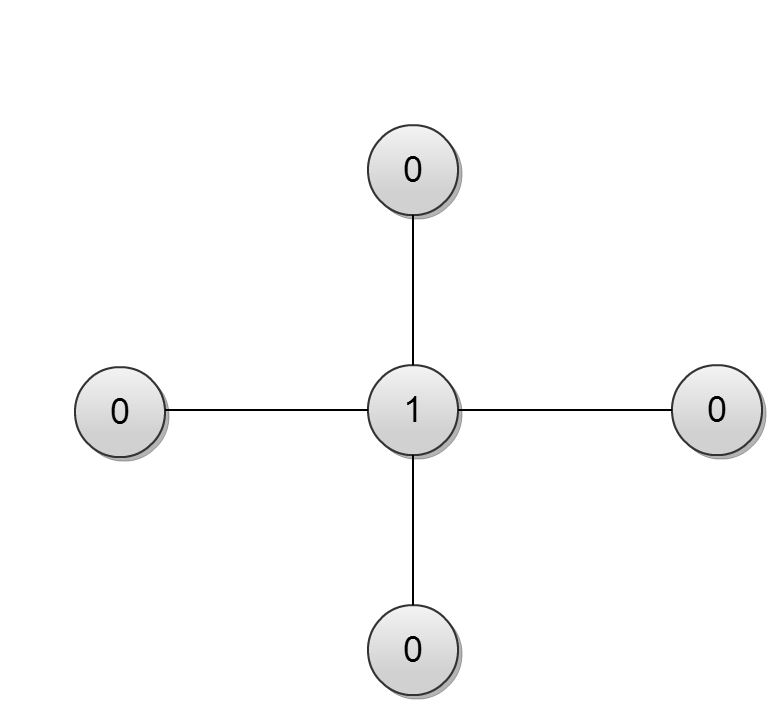
\includegraphics[width=0.8\linewidth]{optimalequilibrium.png}
  \caption{\label{fig:optequi} Socially Optimal equilibrium, center node choose action 1}
\end{subfigure}
\quad
\begin{subfigure}{.4\textwidth}
  \centering
  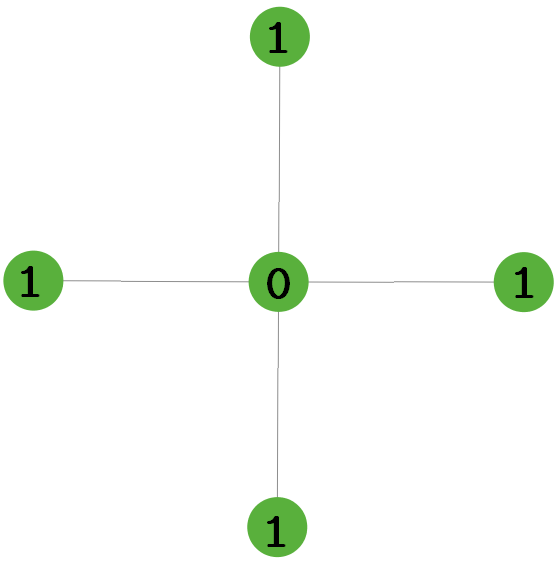
\includegraphics[width=0.8\linewidth]{notoptimalequilibrium.png}
  \caption{\label{fig:notoptequi} Non Socially Optimal equilibrium, leaf nodes choose action 1}
\end{subfigure}
\caption[Socially and non socially optimal equilibrium of a star]{\label{fig:starequi} Figure \ref{fig:optequi} shows the socially optimal equilibrium, and Figure \ref{fig:notoptequi} shows the non optimal equilibrium.}

\end{figure}
Looking at Figure \ref{fig:starequi}, we easily see that there are two equilibriums. One where the center node chooses action 1 and the rest of the nodes choose action 0, and a second equilibrium where all the leaf nodes choose 1 and the center chooses 0.
The overall payoff in these two differs from eachother, the latter is not socially optimal because it
 suffers from a cost equal to: $\#leaf nodes*c$, while the other equilibrium only has a total cost of $c$.
 It would have been beneficial if we were able to force the game to always end up in the socially optimal equilibrium.


\subparagraph{From an insurer's point of view.}
If an insurance company could identify these star structures, and force them to end up in the socially optimal equilibrium, i.e. minimize the overall cost of link establishment, it would have been very beneficial for both the insurer and the customers.
First of all, if the insurer could identify these structures, he could calculate the overall probability of fixation by a contagions node(virus, worm, trojan or other failures). If one could ensure that the center node is protected, one could also calculate the probability of the contagions node being extinguished from the network, and possibly being able to ensure that the network is secure, at least with high probability. 
One possibility of achieving this could be by offering very cheap insurance to the leaf nodes, and giving the center node an incentive to acquire security products by informing the center node about the probability of failure unless he acquires security, and offer him a decent rebate if he acquires the security product, and a very expensive insurance if not. In this way the insurer could force a rational center node into getting both insurance and a security product, and thus increase the security in the whole network.

This is a simple scenario, analyzing an exogenous network formation, but it shows how an insurer can force a star network to end up in the social optimal cost equilibrium. Leading to overall higher security for in the network. We also showed how the insurer could calculate the probabilities of fixation in circulation, star, funnel, meta-funnel and super-star graphs.  Can the insurer force cyber-insurance networks to evolve into any of these structures, and at the same time separate the nodes into trusted and untrusted environments? 
If so, this could contribute significantly to solving the problems of cyber-insurance. The problems of information asymmetry and interdependent risk is reduced. Because, if the insurer knows the network structure, he can calculate the probabilities of failure and catastrophic events. If the network is a star and the insurer can ensure that the center node is secure, the interdependent risk problem is limited to the security of the center node.


\section{Research Question}
Until now, our thesis has introduced cyber-insurance, presented related work on the issues regarding cyber-insurance and this chapter has presented the properties of different graph structures and briefly introduced the idea of network formation. Generally, the papers in the related work section have presented different models for solving the problems with cyber-insurance. Nevertheless, as we have seen, the cyber-insurance market still fails to evolve, despite all the solutions presented in the different papers. This is why we have chosen to take a different approach.
In this chapter, we have shown some structures, especially the star and clique, which could generate benefit for both the insurer and customers in a cyber-insurance market. 
We will combine the knowledge of these structures and network formation games to investigate networks consisting of nodes, insured or not, wanting to increase their payoff by establishing links with eachother. Is it possible for the insurer to force these networks to evolve endogenously into these structures?
We will focus on how the insurer can determine the resulting formation by adjusting the parameter he can control, i.e. the insurance cost. We know that if the insurance premium is too high, no one will buy it. On the other hand, if it is too low, everyone would benefit from having insurance, and insured nodes will make risky decisions, such as connecting to risky nodes. We will try to determine whether it is possible to find the intersections, where the desired structures will evolve, and both the insurer and their customers will benefit from this.


